\rhead{Nicht deterministische Automaten}
\section{Nicht deterministische Automaten\label{regulaer:nea}}
Ein DEA sieht jeweils nur ein Zeichen weit, kann sich nicht an ältere
Zeichen erinnern und kann seine früheren Entscheidungen beim Eintreffen
neuer Zeichen nicht mehr revidieren.
Es ist daher nicht unmittelbar klar,
wie eine Bedingung wie ``wenn ein
Wort mit einer {\tt 0} aufhört, dann muss es auch mit einer {\tt 0}
beginnen'' implementiert werden müsste.

\index{Automat!nicht deterministischer}%
\index{NEA|see{nicht deterministischer endlicher Automat}}%
Nichtdeterminismus erweitert 
die Definition eines endlichen Automaten, um solche Fälle leichter 
zugänglich zu machen.
Es stellt sich daher die Frage, ob die Menge 
der Sprachen, die von solchen nichtdeterministischen endlichen Automaten (NEA)
erkannt werden können,
grösser ist.
Es wird sich zeigen, dass jeder NEA
in einen äquivalenten DEA umgewandelt werden kann, NEAs erkennen also
die gleichen Sprachen wie DEAs.

\subsection{Definition\label{regulaer:definition-nea}}
In einem DEA gibt es zu jedem Zustand $q\in Q$
und jedem Zeichen $a\in\Sigma$ genau
einen Übergang in den Zustand $\delta(q,a)$.
Ein nicht deterministischer Automat lässt dagegen mehrere Möglichkeiten zu.
Das ``Resultat''
von $\delta$ ist also nicht mehr ein (eindeutiger) neuer Zustand, sondern
eine ganze Menge von Zuständen, also ein Element der Potenzmenge $P(Q)$.

Zudem soll ein
nicht deterministischer Automat auch einen Übergang durchführen
können, wenn gar kein Input anliegt.
Ausser den Zeichen aus $\Sigma$ soll für das zweite Argument
von $\delta$ auch das leere Wort zulässig sein.

\begin{definition}\label{definition_nea}
Ein nichtdeterministischer endlicher Automat (NEA) ist ein Quintupel
$(Q,\Sigma,\delta, q_0,F)$ mit
\begin{compactenum}
\item $Q$ ist eine beliebige endliche Menge von Zuständen
\item $\Sigma$ ist eine endliche Menge, genannt das Alphabet.
\item $\delta\colon Q\times(\Sigma\cup\{\varepsilon\})\to P(Q)$ heisst Übergangsfunktion
\item $q_0\in Q$ heisst Startzustand
\item $F\subset Q$ heisst die Menge der Akzeptierzustände.
\end{compactenum}
\end{definition}
\index{$\varepsilon$-Übergänge}%
Übergänge mit $\varepsilon$ als ``Input'' heissen $\varepsilon$-Übergänge.
Ein NEA kann einen solchen Übergang durchführen ``wann er Lust hat''.
Wir bezeichnen NEAs mit $\varepsilon$-Übergängen auch als
NEA$\mathstrut_\varepsilon$.

Ein DEA ist ein Spezialfall eines NEA.
Ein NEA ist ein DEA, wenn
\begin{align}
\delta(q,\varepsilon)&=\emptyset&&\forall q\in Q\label{deanea1}\\
|\delta(q,a)|&=1&&\forall q\in Q, a\in\Sigma\label{deanea2}
\end{align}
Die erste Bedingung (\ref{deanea1}) bedeutet, dass keine
$\varepsilon$-Übergänge vorkommen.
Die zweite Bedingung (\ref{deanea2}) bedeutet, dass von jedem Zustand zu
jedem Zeichen genau ein neuer Zustand möglich ist.

\subsubsection{Gerichteter beschrifteter Graph eines NEA}
\index{Graph!gerichteter!beschrifteter!eines NEA}%
Auch ein NEA kann durch einen gerichteten beschrifteten Graphen
visualisiert werden.
Die Vertizes sind die Zustände $V=Q$.
Die Kanten sind mit Element aus $\Sigma\cup\{\varepsilon\}$ beschriftet.
Von der Ecke $q\in Q$ aus führt zu jedem Element von $\delta(q,a)\in P(Q)$
eine mit $a$ beschriftete Kante, wobei $a\in \Sigma\cup\{\varepsilon\}$, $a=\varepsilon$ ist also auch möglich.

Es ist also durchaus denkbar, dass von einem Zustand $q$ aus für ein
bestimmtes Eingabezeichen $a$ kein Übergang möglich ist, nämlich
wenn $\delta(q,a)=\emptyset$.
Der Automat ``verklemmt'' sich sozusagen in dieser Situation und ist
sicher nicht in der Lage, ein Wort, welches
ihn in diese Situation geführt hat, zu akzeptieren.


\subsection{Beispiele}
\begin{beispiel}[\bf Ganzzahl-Automat]
Im Ganzzahl-Automat führen viele Übergänge zum Zustand $e$, der
alle fehlerhaften Inputs aufsammelt.
Wir könnten diesen Zustand einfach
weglassen und erhalten folgenden, wesentlich übersichtlicheren NEA:
\begin{center}
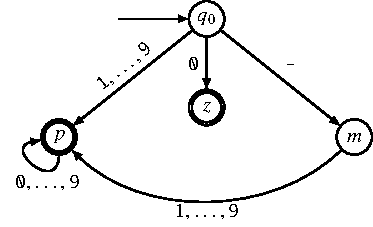
\includegraphics{3-regulaer/images/zahlennea.pdf}
\end{center}
Aus Zustand $q_0$ ist kein Übergang mit dem Zeichen {\tt 0} möglich,
dadurch werden führende Nullen verboten.
Ein {\tt -} kann nur am Anfang
stehen, befindet sich der Automat bereits im Zustand $m$ oder $p$, kann 
er keine weiteren {\tt -} akzeptieren.
Nach einem {\tt -} darf nur ein $\texttt{1}\dots\texttt{9}$ folgen,
denn vom Zustand $m$
aus gibt es keinen mit \texttt{0} angeschrieben Übergang.
\end{beispiel}

\begin{beispiel}[\bf Bedingung an ein einzelnes Zeichen]
Sei $\Sigma=\{{\tt a},{\tt b}\}$, man finde einen NEA, der die 
Sprache akzeptiert, deren Wörter an der drittletzten Stelle
eine {\tt a} haben.
Eine mögliche Lösung ist der Automat
\begin{center}
\begin{tikzpicture}[>=latex,thick]
\coordinate (q0) at (0,0);
\coordinate (q1) at (2,0);
\coordinate (q2) at (4,0);
\coordinate (q3) at (6,0);

\draw (q0) circle[radius=0.35];
\draw (q1) circle[radius=0.35];
\draw (q2) circle[radius=0.35];
\draw (q3) circle[radius=0.35];
\draw (q3) circle[radius=0.3];

\node at (q0) {$q_0$};
\node at (q1) {$q_1$};
\node at (q2) {$q_2$};
\node at (q3) {$q_3$};

\draw[->,shorten >= 0.35cm,shorten <= 0.35cm] (-2,0) -- (q0);
\draw[->,shorten >= 0.35cm,shorten <= 0.35cm] (q0) -- (q1);
\draw[->,shorten >= 0.35cm,shorten <= 0.35cm] (q1) -- (q2);
\draw[->,shorten >= 0.35cm,shorten <= 0.35cm] (q2) -- (q3);
\draw[->,shorten >= 0.35cm,shorten <= 0.35cm]
	(q0) to[out=-60,in=-120,distance=1.3cm] (q0);

\node at ($0.5*(q0)+0.5*(q1)$) [above] {\texttt{a}};
\node at ($0.5*(q1)+0.5*(q2)$) [above] {\texttt{a},\texttt{b}};
\node at ($0.5*(q2)+0.5*(q3)$) [above] {\texttt{a},\texttt{b}};
\node at ($(q0)+(0,-1)$) [below] {\texttt{a},\texttt{b}};

\end{tikzpicture}
\end{center}
Der Automat ist nicht deterministisch, weil im Zustand $q_0$ zwei verschiedene
Übergänge für das Zeichen {\tt a} möglich sind.
Der Automat bleibt
sozusagen im Zustand $q_0$ bis er ``weiss'', dass jetzt das drittletzte
Zeichen ansteht.
\end{beispiel}

\begin{beispiel}[\bf Teilbarkeit]
Für $\Sigma=\{{\tt 0}\}$ finde einen NEA für die Sprache 
\[
L=\{w\in \Sigma^*\;|\; \text{$|w|$ ist durch 2 oder 3 teilbar}\}.
\]
Das Problem bei der Konstruktion eines DEA ist, dass wird zu
Beginn noch nicht wissen können, ob wir einen ankommenden
String auf Teilbarkeit durch $2$ oder durch $3$ testen sollen.
Also verwenden wir $\varepsilon$-Übergänge aus dem Startzustand
in zwei verschiedene Automaten, die die Teilbarkeit testen:
\begin{center}
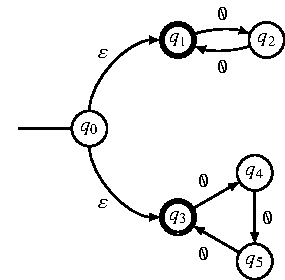
\includegraphics{3-regulaer/images/teilbarkeit.pdf}
\end{center}
\end{beispiel}

\subsection{Erreichbare Zustände\label{regulaer:erreichbarezustaende}}
\index{erreichbare Zustände}%
Im Folgenden werden wir berechnen müssen, welche Menge von Zuständen
durch einen Übergang oder mehrere verkettete Übergänge erreicht werden
können.
Es besteht ein Unterschied, ob der Übergang infolge eines
Input-Zeichens $a\in\Sigma$ erfolgt, oder ob er spontan als
$\varepsilon$-Übergang ausgeführt werden kann.

\subsubsection{Übergang zu Zeichen aus $\Sigma$}
Die Menge $\delta(q,a)\subset Q$ gibt die in einem Schritt mit Inputzeichen $a$
von $q$ aus erreichbaren Zustände von $Q$ an.
Für den Input $a_1a_2$ kann
man von jedem Zustand in $\delta(q,a_1)$ aus weiter Zustände mit einem
Überang mit Inputzeichen $a_2$ erreichen.
Die Menge der erreichbaren Zustände ist
\begin{equation}
\delta(q,a_1a_2)=\bigcup_{q_1\in\delta(q,a_1)}\delta(q_1, a_2)
=\delta(\delta(q,a_1),a_2)
\label{erreichbar}
\end{equation}
Dies kann man wiederholen:
\begin{align*}
\delta(q,a_1a_2a_3)&=
\bigcup_{q_2\in\delta(q, a_1a_2)}\delta(q_2,a_3)
=
\delta(\delta(\delta(q,a_1),a_2),a_3)
\\
\delta(q,a_1\dots a_n)&=\bigcup_{q_{n-1}\in\delta(q,a_1\dots a_{n-1})}\delta(q_{n-1},a_n)
=\delta(\dots \delta(q,a_1)\dots,a_n)
\end{align*}
Die so definierte Menge $\delta(q,a_1\dots a_n)$ umfasst alle von
$q$ aus erreichbaren Zustände.

Falls $q'\in\delta(q,a_1\dots a_n)$ gibt
es insbesondere eine Folge von Zwischenzuständen $q_1,\dots,q_{n-1}$
mit $q_k\in\delta(q_{k-1},a_k)$ für alle $k$.
Ausserdem  ist natürlich $q_k\in\delta(q,a_1\dots a_k)$ für alle $k$.

Eine Menge $M$ von Zuständen stellt man sich am besten vor, indem man die
darin enthaltenen Zustände farbig markiert.
In der Menge $\delta(M,a)$ befinden sich alle Zustände, die von Zuständen
von $M$ aus mit Input $a$ erreichbar sind.

\subsubsection{$\varepsilon$-Übergänge}
Einzelne Zustände kann man auch durch $\varepsilon$-Übergänge
erreichen.
Die Menge der Zustände, die von $q\in Q$ aus durch
$\varepsilon$-Übergänge erreichbar sind, bezeichnen wir mit
$E(q)$.
Sie setzt sich zusammen aus Zuständen, die in einem einzigen 
Schritt erreichbar sind, und solchen, die durch wiederholte
Schritte erreichbar werden.
\[
E(q)=\{q\} \cup \delta(q,\varepsilon) \cup \delta(\delta(q,\varepsilon),\varepsilon)\cup\dots
\]

\subsection{''Könnte''-Automat\label{Thompson-NEA}}
Ein NEA hat bei jedem Übergang eventuell mehrere Zielstände zur Auswahl.
Eine Implementation muss im Prinzip alle diese Möglichkeiten 
durchprobieren.
Alternativ könnte er sich aber auch merken,
welche möglichen Zustände im Laufe der Verarbeitung eines
Wortes erreicht werden konnten.
Die Menge der möglichen erreichten Zustände kann mit jedem
neuen Zeichen des Inputwortes neu berechnet werden.
Eine separate Speicherung ist nicht erforderlich, wenn man die
erreichten Zustände mit einer Markierung versieht.

\begin{figure}
\begin{center}
\includegraphics{images/reg-2}
\end{center}
\caption{Beispiel eines NEA\label{koenntenea}}
\end{figure}

\begin{figure}
\begin{center}
\begin{tabular}{cccc}
&%
\includegraphics{images/reg-2}&
\raisebox{60pt}{$\overset{\displaystyle\text{\tt b}}\longrightarrow$}&
\includegraphics{images/reg-3}\\
\raisebox{60pt}{$\overset{\displaystyle\text{\tt a}}\longrightarrow$}&
\includegraphics{images/reg-4}&
\raisebox{60pt}{$\overset{\displaystyle\text{\tt a}}\longrightarrow$}&
\includegraphics{images/reg-5}
\end{tabular}
\end{center}
\caption{Verarbeitung des Wortes {\tt baa} durch den NEA von
Abbildung~\ref{koenntenea}.
Die möglichen Zustände sind jeweils
rot markiert.\label{koenntebeispiel}
}
\end{figure}
Abbildung~\ref{koenntenea} zeigt einen NEA mit drei Zuständen.
Wir verfolgen die Verarbeitung des Wortes {\tt baa} in
Abbildung~\ref{koenntebeispiel}.

Bevor ein Zeichen verarbeitet wird,
ist der NEA im Startzustand $q_0$, also ist genau dieser Zustand
markiert.
Die Verarbeitung des Zeichens {\tt b} ist deterministisch,
sie bringt den NEA in den Zustand $q_1$.
Das folgende Zeichen {\tt a}
ist jedoch nicht mehr deterministisch, es sind sowohl $q_1$ als auch
$q_2$ als Folgezustände möglich.
Die markierte mögliche Menge von Zuständen nach Verarbeitung von {\tt ba}
ist daher $\{q_1,q_2\}$.
Bei der Verarbeitung des zweiten {\tt a} kommt noch der Zustand $q_0$ hinzu.
Man berechnet also schrittweise die
Menge der erreichbaren Zustände $\delta(q_0,{\tt baa})$.

Nach Verarbeitung des ganzen Wortes kann der NEA in den Zuständen
$\{q_0,q_1,q_2\}$ sein.
Da der Akzeptierzustand $q_0$ in dieser Menge
enthalten ist, gibt es eine Kombination von nichtdeterministischen
Entscheidungen, die zu $q_0$ führen, das Wort {\tt baa} kann also
akzeptiert werden.

\index{Thompson, Ken}%
\index{Thompson-NEA}%
Diese Implementation eines NEA geht auf Ken Thompson zurück, sie wurde in
der Regex-Library der achten Edition von Unix von Rob Pike
\index{Pike, Rob}%
implementiert, die allerdings nicht sehr weit verbreitet war.
Später hat Henry Spencer die Regex-Library neu
implementiert, allerdings ohne die Thompson-NEA Konstruktion, sondern
mit Backtracking.
Da er sie in den public domain freigab, hat sie sich
rasch verbreitet und bildete die Basis Regex-Bibliotheken in Perl, PCRE,
Python und vielen anderen.

\subsection{Transformation NEA \texorpdfstring{$\rightarrow$}{->} DEA\label{regulaer:nea-dea}}
NEAs führen trotz der beträchtlichen Erweiterung durch den
Nichtdeterminismus nicht zu einer grösseren Klasse von akzeptierbaren
Sprachen.
Dazu genügt es zu zeigen, dass sich jeder NEA in einen DEA
transformieren lässt, der die gleiche Sprache akzeptiert.
Dass dies möglich sein sollte, deutet bereits die Konstruktion
des Thompson-NEA in \ref{Thompson-NEA} an.
Der Thompson-NEA wird zu einem DEA, wenn man die Verteilung der
``roten Markierungen'' als Zustand des DEA ansieht.
Ziel dieses Abschnittes ist, dies
mathematisch streng zu formalisieren.

Ein NEA kann aus zwei Gründen kein DEA sein:
er kann $\varepsilon$-Übergänge haben und er kann nicht eindeutige
oder nicht existierende Übergänge haben, also $|\delta(q,a)|\ne 1$
für gewisse $q\in Q$ und $a\in\Sigma$.
Wir transformieren einen 
beliebigen NEA in zwei Schritten in einen DEA:
\begin{enumerate}
\item Wir bauen uns einen Algorithmus, mit dem man einen NEA ohne
$\varepsilon$-Übergänge in einen DEA umwandeln kann.
\item Wir modifizieren den Algorithmus, so dass er auch mit NEAs mit
$\varepsilon$-Übergängen umgehen kann.
\end{enumerate}

\subsubsection{Transformation für NEA ohne $\varepsilon$-Übergänge}
Der konstruierte DEA muss darüber Buch führen, in welchen Zuständen
der NEA sein könnte.
Seine Zustände sind als Mengen von möglichen Zuständen des NEA.
Als Zustandsmenge des DEA wird man also $P(Q)$ 
erwarten.
Wie die übrigen Elemente des DEA konstruiert werden müssen,
besagt der folgende Satz.

\begin{satz}
\label{satz_neadea_eps}
Sei $A=(Q,\Sigma,\delta,q_0,F)$ ein NEA ohne $\varepsilon$-Übergänge.
Dann gibt es einen DEA $A'$, der die gleiche Sprache akzeptiert: $L(A)=L(A')$.
Der DEA $A'$ setzt sich zusammen aus
\[
A'=
(P(Q), \Sigma, \delta', \{q_0\}, F'),
\]
die Übergangsfunktion ist
\[
\delta'\colon P(Q)\times \Sigma: (M, a)\mapsto \bigcup_{q\in M} \delta(q,a)
=\delta(M,a),
\]
und die Akzeptierzustände sind die Teilmengen, die einen Akzeptierzustand
enthalten:
\[
F'=\{M\in P(Q)\;|\;M\cap F\ne \emptyset\}.
\]
\end{satz}
\begin{proof}[Beweis]
Es ist klar, dass mit dieser Übergangsfunktion $\delta'$ und den
Akzeptierzuständen $F'$ ein DEA definiert ist, es muss nur noch
bewiesen werden, dass er die gleiche Sprache akzeptiert, also
$L(A)=L(A')$.
Das wird zutreffen, wenn $L(A)\subset L(A')$ und
$L(A')\subset L(A)$, also jedes Wort von $L(A)$ ist auch in $L(A')$,
und umgekehrt.

Wenn $w=a_1\dots a_n\in L(A)$, dann gibt es einen Pfad durch den gerichteten
Graphen von $A$, der zu einem Akzeptierzustand führt.
Also enthält
die Menge der von $q_0$ aus erreichbaren Zustände einen Akzeptierzustand.
Diese Menge ist aber die Menge der Zustände, die man durch Anwendung
von $\delta'$ aus $\{q_0\}$ und den Inputzeichen $a_1,\dots,a_n$ erhalten
wird.
Da diese Menge einen Akzeptierzustand enthält, ist sie ein
Akzeptierzustand von $A'$ und damit $w\in L(A')$.

Sei jetzt umgekehrt $w\in L(A')$.
Wir schreiben wieder $w=a_1\dots a_n$.
Auf Grund der Konstruktion des Automaten $A'$, liefert die wiederholte
Anwendung von $\delta'(\cdot, a_k)$ aus dem Anfangszustand $q_0'=\{q_0\}$
die Menge $\delta(\dots\delta(q_0, a_1)\dots ,a_n)$.
Da diese Menge ein
Akzeptierzustand von $A'$ ist, gibt es darin einen Akzeptierzustand
von $A$.
Da also ein Akzeptierzustand erreichbar ist, ist $w\in L(A)$,
also auch $L(A')\subset L(A)$.
\end{proof}

\subsubsection{Beispiel}
Der NEA von Abbildung~\ref{koenntenea}
%\[
%\entrymodifiers={++[o][F]}
%\xymatrix{
%*+\txt{}\ar[r]
%	&*++[o][F=]{q_0} \ar[d]_{\tt b} 
%		&{q_2}\ar[l]_{\tt a}
%\\
%*+\txt{}
%	&{q_1}\ar[ur]_{{\tt a},{\tt b}} \ar@(ul,dl)_{\tt a}
%}
%\]
soll in einen DEA umgewandelt werden.
Er ist nicht deterministisch,
weil vom Zustand $q_1$ aus zwei Übergänge mit {\tt a} möglich sind.

Aus dem Satz ist bekannt, dass die Zustände die Potenzmengen von $Q$ sind.
Diese entsprechen den dreistelligen Binärzahlen, wobei jede
Stelle angibt, ob das zugehörige $q_i$ in der Menge dabei ist.
Wir
schreiben also
\begin{align*}
       &          &q_{001}&=\{\phantom{q_2q_1}q_0\}&q_{110}&=\{q_2,q_1\phantom{,q_0}\}&&\\
q_{000}&=\emptyset&q_{010}&=\{\phantom{q_2}q_1\phantom{q_0}\}&q_{101}&=\{q_2,\phantom{q_1,}q_0\}&q_{111}&=\{q_2,q_1,q_0\}\\
       &          &q_{100}&=\{q_2\phantom{q_1q_0}\}&q_{011}&=\{\phantom{q_2,}q_1,q_0\}&&\\
\end{align*}
Akzeptierzustände sind jene Mengen, die $q_0$ enthalten, also
\[
F'=\{ q_{001}, q_{011}, q_{101}, q_{111}\},
\]
Startzustand ist $q_{001}$.
Damit können wir jetzt das Zustandsdiagramm zeichnen
\[
\entrymodifiers={++[o][F]}
\xymatrix{
*+\txt{}\ar[r]
	&*++[o][F=]{q_{001}} \ar[d]^{\tt b}\ar[dl]_{\tt a}
		&{q_{110}}\ar[dr]^{\tt a} \ar[ddl]^{\tt b}
\\
{q_{000}}\ar@(ul,dl)_{{\tt a},{\tt b}}
	&{q_{010}} \ar[ur]^{\tt a} \ar[d]^{\tt b}
		&*++[o][F=]{q_{101}} \ar[ul]^{\tt a} \ar[l]^{\tt b}
			&*++[o][F=]{q_{111}}\ar@(ur,dr)^{{\tt a}} \ar@/_20pt/[ul]_{\tt b}
\\
*+\txt{}
	&{q_{100}}\ar@/^20pt/[uu]^{\tt a}  \ar[ul]^{\tt b}
		&*++[o][F=]{q_{011}} \ar@/_20pt/[uu]_{{\tt a},{\tt b}}
}
\]
Man erkennt sofort, dass die Zustände $q_{101}$ und $q_{011}$
nicht erreicht werden können, also weggelassen werden könnten:
\begin{equation}
\entrymodifiers={++[o][F]}
\xymatrix{
*+\txt{}\ar[r]
	&*++[o][F=]{q_{001}} \ar[d]^{\tt b}\ar[dl]_{\tt a}
		&{q_{110}}\ar[dr]^{\tt a} \ar[ddl]^{\tt b}
\\
{q_{000}}\ar@(ul,dl)_{{\tt a},{\tt b}}
	&{q_{010}} \ar[ur]^{\tt a} \ar[d]^{\tt b}
		&*+\txt{}
			&*++[o][F=]{q_{111}}\ar@(ur,dr)^{{\tt a}} \ar@/_20pt/[ul]_{\tt b}
\\
*+\txt{}
	&{q_{100}}\ar@/^20pt/[uu]^{\tt a}  \ar[ul]^{\tt b}
		&*+\txt{}
}
\label{nea-eps}
\end{equation}
Man kann ebenfalls verifzieren, dass dies tatsächlich ein DEA ist, 
von jedem Zustand gehen genau zwei Pfeile für die Übergänge mit
den Zeichen ${\tt a}$ und ${\tt b}$ aus.
Etwas übersichtlicher geschrieben lautet er
\[
\entrymodifiers={++[o][F]}
\xymatrix{
*+\txt{}\ar[r]
	&*++[o][F=]{1}\ar[r]^{\tt b} \ar[d]_{\tt a}
		&2 \ar[r]^{\tt a} \ar[d]^{\tt b}
			&6\ar@/_/[r]_{\tt a} \ar[dl]^{\tt b}
				&*++[o][F=]{7}\ar@/_/[l]_{\tt b} \ar@(ur,dr)^{\tt a}
\\
*+\txt{}
	&0 \ar@(l,d)_{{\tt a},{\tt b}}
		&4 \ar[ul]_{\tt a} \ar[l]^{\tt b}
}
\]

\subsubsection{NEA mit $\varepsilon$-Übergängen}
Wir erweitern die Konstruktion des DEA aus einem NEA jetzt, um eventuell
vorhandenen $\varepsilon$-Übergängen Rechnung zu tragen.

\begin{satz}
\label{satz_neadea}
Sei $A=(Q,\Sigma,\delta,q_0,F)$ ein NEA, dann gibt es einen
DEA $A'=(Q',\Sigma,\delta',q_0',F')$, der die gleiche Sprache
akzeptiert, $L(A)=L(A')$.
Es ist
\begin{align*}
Q'&=P(Q)\\
\delta'(M,a)&=E(\delta(M, a))\quad M\in P(Q)\\
q_0'&=E(q_0)\\
F'&=\{M\in P(Q)\;|\, M\cap F\ne \emptyset\}
\end{align*}
\end{satz}

\begin{proof}[Beweis]
Gegenüber Satz \ref{satz_neadea} hat sich geändert, dass wir den
Anfangszustand von $\{q_0\}$ auf $E(q_0)$ vergrössert haben.
Dadurch erfassen wir alle Pfade durch den Automaten, die mit einem oder
mehreren $\varepsilon$-Übergängen beginnen.
Falls $E(q_0)\cap F\ne \emptyset$
wird der Anfangszustand auch zu einem Endzustand.

Zudem erweitern wir in der Definition des Bildes $\delta(M,a)$ um alle Zustände,
die durch einen angehängten $\varepsilon$-Übergang erreicht werden
können.
\end{proof}

\subsubsection{Beispiel}
Der NEA 
\[
\entrymodifiers={++[o][F]}
\xymatrix{
*+\txt{}\ar[r]
	&*++[o][F=]{q_0} \ar[d]_{\tt b} \ar@/_/[r]_{\varepsilon}
		&{q_2}\ar@/_/[l]_{\tt a}
\\
*+\txt{}
	&{q_1}\ar[ur]_{{\tt a},{\tt b}} \ar@(ul,dl)_{\tt a}
}
\]
soll in einen DEA umgewandelt werden.

Den NEA ohne den $\varepsilon$-Übergang haben wir bereits in
\ref{nea-eps} umgewandelt.
Jetzt müssen wir nur die beiden
im Satz \ref{satz_neadea} erwähnten Modifikationen durchführen.

Ursprünglich war der Startzustand $q_{001}$.
Da aus dem Startzustand
des NEA mittels $\varepsilon$-Übergang auch der Zustand $q_2$
erreichbar ist, muss der Anfangszustand des DEA um diesen Zustand
erweitert werden und ist jetzt $q_{101}$:
\[
\entrymodifiers={++[o][F]}
\xymatrix{
*+\txt{}
	&*++[o][F=]{q_{001}} \ar[d]^{\tt b}\ar[dl]_{\tt a}
		&{q_{110}}\ar[dr]^{\tt a} \ar[ddl]^{\tt b}
\\
{q_{000}}\ar@(ul,dl)_{{\tt a},{\tt b}}
	&{q_{010}} \ar[ur]^{\tt a} \ar[d]^{\tt b}
		&*++[o][F=]{q_{101}} \ar[ul]^{\tt a} \ar[l]^{\tt b}
			&*++[o][F=]{q_{111}}\ar@(ur,dr)^{{\tt a}} \ar@/_20pt/[ul]_{\tt b}
\\
*+\txt{}
	&{q_{100}}\ar@/^20pt/[uu]^{\tt a} \ar[ul]^{\tt b}
		&*++[o][F=]{q_{011}} \ar@/_20pt/[uu]_{{\tt a},{\tt b}}
			&*+\txt{}\ar[ul]
}
\]


Zusätzlich müssen wir bei jedem Übergang die Möglichkeit in
Betracht ziehen, dass noch ein $\varepsilon$-Übergang angehängt
wird.
Dies bedeutet im vorliegenden Fall, dass bei jedem Übergang,
der zu einem $q_0$ enthaltenden Zustand führt, auch noch der
Zustand $q_2$ hinzugefügt werden muss.
\[
\entrymodifiers={++[o][F]}
\xymatrix{
*+\txt{}
	&*++[o][F=]{q_{001}} \ar[d]^{\tt b}\ar[dl]_{\tt a}
		&{q_{110}}\ar[dr]^{\tt a} \ar[ddl]^{\tt b}
\\
{q_{000}}\ar@(ul,dl)_{{\tt a},{\tt b}}
	&{q_{010}} \ar[ur]^{\tt a} \ar[d]^{\tt b}
		&*++[o][F=]{q_{101}} \ar@(ul,ur)^{\tt a} \ar[l]^{\tt b}
			&*++[o][F=]{q_{111}}\ar@(ur,dr)^{{\tt a}} \ar@/_20pt/[ul]_{\tt b}
\\
*+\txt{}
	&{q_{100}}\ar[ur]^{\tt a} \ar[ul]^{\tt b}
		&*++[o][F=]{q_{011}} \ar@/_20pt/[uu]_{{\tt a},{\tt b}}
			&*+\txt{}\ar[ul]
}
\]
In diesem Automaten sind die Zustände $q_{001}$ und $q_{011}$ nicht
mehr erreichbar, man kann sie weglassen.
\[
\entrymodifiers={++[o][F]}
\xymatrix{
*+\txt{}
	&*+\txt{}
		&{q_{110}}\ar[dr]^{\tt a} \ar[ddl]^{\tt b}
\\
{q_{000}}\ar@(ur,dr)^{{\tt a},{\tt b}}
	&{q_{010}} \ar[ur]^{\tt a} \ar[d]^{\tt b}
		&*++[o][F=]{q_{101}} \ar@(ul,ur)^{\tt a} \ar[l]^{\tt b}
			&*++[o][F=]{q_{111}}\ar@(ur,dr)^{{\tt a}} \ar@/_20pt/[ul]_{\tt b}
\\
*+\txt{}
	&{q_{100}}\ar[ur]^{\tt a} \ar[ul]^{\tt b}
		&*+\txt{}
			&*+\txt{}\ar[ul]
}
\]
Wie man mit dem Algorithmus über den Minimalautomaten kontrollieren
kann, lässt sich dieser Automat nicht mehr weiter reduzieren.
Etwas übersichtlicher geschrieben lautet er
\[
\entrymodifiers={++[o][F]}
\xymatrix{
*+\txt{}\ar[r]
	&*++[o][F=]{5}\ar@(ul,ur)^{\tt a} \ar[r]^{\tt b}
		&2\ar[r]^{\tt a} \ar[d]^{\tt b}
			&6\ar@/_/[r]_{\tt a} \ar[dl]^{\tt b}
				&*++[o][F=]{7}\ar@/_/[l]_{\tt b} \ar@(ur,dr)^{\tt a}
\\
*+\txt{}
	&0\ar@(ul,dl)_{{\tt a},{\tt b}}
		&4\ar[ul]^{\tt a} \ar[l]^{\tt b}
}
\]


Satz \ref{satz_neadea} ist nicht nur ein theoretisch interessantes
Resultat.
Wenn man die endliche vielen Zustände mit den Zahlen
$0,\dots,|Q|-1$ identifiziert, kann man die Teilmengen von $Q$ mit
den $|Q|$-stelligen Binärzahlen identifizieren.
Der Teilmenge $M\subset Q$ entsprechen die Binärzahlen, die Einsen an
den Stellen haben, deren Nummern in $M$ enthalten sind.
Die grosse Vereinigungen ist ebenfalls sehr einfach
zu berechnen, sie entspricht der Oder-Verknüpfung
der einzelnen Mengen in (\ref{erreichbar}).
Somit haben wir nicht nur ein Existenz-Resultat, sondern einen
Algorithmus, mit dem ein beliebiger NEA in einen DEA umgewandelt
werden kann.
Daraus können wir jetzt einen Vergleichsalgorithmus für reguläre
Sprachen ableiten: 

\begin{satz}
Es gibt einen Algorithmus, mit dem entschieden werden kann, ob
zwei Automaten $A$ und $B$ die gleiche Sprache akzeptieren.
\end{satz}

\begin{proof}[Beweis]
Um zu entscheiden, ob $L(A)=L(B)$, wendet man folgenden Algorithmus
an:
\begin{enumerate}
\item Wandle $A$ und $B$
mit dem Algorithmus des Satzes 
\ref{satz_neadea} in die DEAs $A'$ und $B'$ um.
\item Reduziert anschliessend $A'$ und $B'$  mit dem Algorithmus
von Satz \ref{satz_minimalautomat} in Minimalautomaten
$A''$ und $B''$.
\item Die von $A$ und $B$ akzeptierten Sprachen sind genau dann
gleich, wenn $A''$ und $B''$ identisch sind.
\end{enumerate}
\end{proof}

Der hier vorgeschlagene Beweis ist allerdings oft nicht praktikabel.
Der aus dem NEA erzeugte DEA hat im schlechtesten Fall $2^n$
Zustände, wenn der NEA $n$ Zustände hatte, die Laufzeit des
Algorithmus ist also exponentiell in der Grösse des NEA.
Ein wesentlich schnellerer Algorithmus wurde 2015 von Bonchi und Pous
gefunden \cite{skript:bonchi-pous}.

\subsection{Mengenoperationen\label{regulaer:mengenoperationen}}
\index{Mengenoperationen}%
\index{Durchschnitt}%
\index{Vereinigung}%
\index{Differenz}%
Sprachen sind Mengen von Wörtern, also sind auch deren Vereinigung,
Durchschnitt, Differenz usw.~Sprachen.
Sind die Sprachen regulär,
sind dann auch Vereinigung, Durchschnitt, Differenz etc.~regulär? 
NEAs erlauben uns sehr elegant zu zeigen, dass Sie diese Operationen
alle wieder reguläre Sprachen liefern.

\begin{satz}
\index{Vereinigung}%
\label{satz_union}
Sind $L_1$ und $L_2$ reguläre Sprachen, dann
ist auch $L_1\cup L_2$ regulär.
\end{satz}

\begin{figure}
\begin{center}
\includegraphics{images/nea-5}
\qquad \qquad
\includegraphics{images/nea-6}
\end{center}
\caption{Konstruktion eines NEA 
für die Sprache $L(A_1)\cup L(A_2)$.\label{regulaer:vereinigung}}
\end{figure}

\begin{proof}[Beweis]
Da die Sprachen regulär sind, gibt es endliche Automaten 
\begin{align*}
A_1&=(Q_1,\Sigma_1,\delta_1, q_{01}, F_1)\\
A_2&=(Q_2,\Sigma_2,\delta_2, q_{02}, F_2)
\end{align*}
mit $L_1=L(A_1)$ und $L_2=L(A_2)$.
Wir müssen
jetzt einen Automaten
\[
A = (Q, \Sigma, \delta, q_0, F)
\]
konstruieren, der $L_1\cup L_2$ akzeptieren
(Abbildung~\ref{regulaer:vereinigung}).

Für die Vereinigung muss das Alphabet alle Zeichen enthalten,
also $\Sigma = \Sigma_1\cup\Sigma_2$.
Man kann jeden der Automaten 
$A_1$ und $A_2$ auch als Automaten über dem Alphabet $\Sigma$
betrachten, indem man setzt
\[
\delta_i(q, x)=\begin{cases}
\delta_i(q,x)&\qquad q\in Q_i\text{ und } x\in \Sigma_i\\
\emptyset&\qquad q\in Q_i\text{ und } x\in \Sigma_{3-i}\setminus \Sigma_i\\
\end{cases}
\]
Es ist also keine Einschränkung, wenn wir annehmen, dass
$\Sigma=\Sigma_1=\Sigma_2$.

Um den Automaten für $L_1\cup L_2$ zu konstruieren, nehmen wir jetzt
weiter an, dass $Q_1$ und $Q_2$ disjunkt sind.
Für $A$ verwenden wir einen neuen Startzustand $q_0$.
Ein Wort in $L_1\cup L_2$ muss von einem der beiden Automaten
akzeptiert werden.
Der Automat muss sich also zu Beginn nichtdeterministisch
dafür entscheiden, den einen oder anderen Automaten zum
akzeptieren eines Wortes zu verwenden.
Also verwenden wir 
\begin{align*}
Q&=Q_1\cup Q_2\cup \{q_0\}\\
F&=F_1\cup F_2\\
\delta(x,a)&=\begin{cases}
\delta_1(x,a)&\qquad x\in Q_1\\
\delta_2(x,a)&\qquad x\in Q_2\\
\{q_{01}, q_{02}\}&\qquad x=q_0, a=\varepsilon\\
\emptyset&\qquad x=q_0, a\ne\varepsilon
\end{cases}
\end{align*}
\end{proof}

\begin{satz}
\index{Durchschnitt}%
\label{satz_intersection}
Sind $L_1$ und $L_2$ reguläre Sprachen, dann
ist auch $L_1\cap L_2$ regulär.
\end{satz}

\begin{proof}[Beweis]
Da die Sprachen regulär sind, gibt es endliche Automaten 
\begin{align*}
A_1&=(Q_1,\Sigma_1,\delta_1, q_{01}, F_1)\\
A_2&=(Q_2,\Sigma_2,\delta_2, q_{02}, F_2)
\end{align*}
mit $L_1=L(A_1)$ und $L_2=L(A_2)$.
Wir müssen jetzt einen Automaten
\[
A = (Q, \Sigma, \delta, q_0, F)
\]
konstruieren, der $L_1\cap L_2$ akzeptiert.

Für die Schnittmenge brauchen wir einen Automaten, der die Abläufe 
in beiden Teilautomaten gleichzeitig codiert.
Dies ist möglich, indem man Zustände und Übergänge nebeneinander
simuliert.
Als Zustandsmenge verwenden wir daher $Q=Q_1\times Q_2$.
Als Übergangsfunktion verwenden wir
\[
\delta((q',q''),a)=\delta_1(q',a)\times \delta_2(q'',a).
\]
Akzeptiert werden kann ein Wort, wenn beide Komponenten des Paares 
Akzeptierzustände ihrer Automaten sind.
Akzeptierzustände von $A$ sind also $F=F_1\times F_2$.
\end{proof}

\index{Produktautomat}%
Wir nennen diesen mit Hilfe des kartesischen Produktes konstruierten
Automaten auch den
{\em kartesischen Produktautomaten}\label{reg_produktautomat}.

\subsubsection{Beispiel}
Zur Illustration wollen 
wir einen Automaten für die Schnittmenge von
\begin{align*}
L_1&=\{w\in\Sigma^*\;|\; \text{$|w|_0$ gerade}\}\qquad\text{und}\\
L_2&=\{w\in\Sigma^*\;|\,\text{$w$ ist eine durch 3 teilbare Binärzahl}\}.
\end{align*}
konstruieren.
Die einzelnen Teilautomaten sind $A_1$ für $L_1$:
\[
\entrymodifiers={++[o][F]}
\xymatrix{
*+\txt{}\ar[r]
	&*++[o][F=]{} \ar@/^/[r]^{\tt 0} \ar@(ul,ur)^{\tt 1}
		&{} \ar@/^/[l]^{\tt 0} \ar@(ul,ur)^{\tt 1}
}
\]
und $A_2$ für $L_2$
\[
\entrymodifiers={++[o][F]}
\xymatrix{
*+\txt{}\ar[r]
	&*++[o][F=]{0} \ar@/^/[r]^{\tt 1} \ar@(ul,ur)^{\tt 0}
		&{1} \ar@/^/[l]^{\tt 1} \ar@/^/[r]^{\tt 0}
			&{2}\ar@(ur,dr)^{\tt 1} \ar@/^/[l]^{\tt 0}
}
\]
Der Produktautomat ist jetzt
\[
\entrymodifiers={++[o][F]}
\xymatrix{
*+\txt{} \ar[r] \ar[d] \ar[dr]
	&*++[o][F=]{0} \ar@/^/[r]_{\tt 1} \ar@(ul,ur)^{\tt 0}
		&{1} \ar@/^/[l] \ar@/^/[r]_{\tt 0}
			&{2}\ar@(ur,dr)^{\tt 1} \ar@/^/[l]
\\
*++[o][F=]{} \ar@/^/[d] \ar@(ul,dl)_{\tt 1}
	&*++[o][F=]{} \ar@/^/[d]{\tt 0} \ar@/^/[r]_{\tt 1}
		&{} \ar@/^/[l] \ar@/^/[dr]_{\tt 0}
			&{}\ar@(ur,dr)^{\tt 1} \ar@/^/[dl]
\\
{} \ar@/^/[u]_{\tt 0} \ar@(ul,dl)_{\tt 1}
	&{} \ar@/^/[u]_{\tt 0} \ar@/^/[r]_{\tt 1}
		&{} \ar@/^/[l] \ar@/^/[ur]
			&{}\ar@(ur,dr)^{\tt 1} \ar@/^/[ul]
}
\]

Man kann den Produktautomaten auch
verwenden, um einen Automaten zu bauen, der $L_1\cup L_2$
akzeptiert.
Der kartesische Produktautomat simuliert ja sozusagen
beide Teilautomaten in den beiden Komponenten der Zustände.
Akzeptabel ist ein Wort $w$, wenn es von $A_1$
oder von $A_2$ akzeptiert ist, oder wenn der Produktautomat
sich am Ende des Wortes in einem Zustand befindet, der ein
Akzeptierzustand von $A_1$ ist oder von $A_2$.
Verwendet
man also $F_1\times Q_2\cup Q_1\times F_2$ als Akzeptierzustände,
erhält man einen Automaten, der $L_1\cup L_2$ akzeptiert.
Das zugehörige Zustandsdiagramm ist:
\[
\entrymodifiers={++[o][F]}
\xymatrix{
*+\txt{} \ar[r] \ar[d] \ar[dr]
	&*++[o][F=]{0} \ar@/^/[r]_{\tt 1} \ar@(ul,ur)^{\tt 0}
		&{1} \ar@/^/[l] \ar@/^/[r]_{\tt 0}
			&{2}\ar@(ur,dr)^{\tt 1} \ar@/^/[l]
\\
*++[o][F=]{} \ar@/^/[d] \ar@(ul,dl)_{\tt 1}
	&*++[o][F=]{} \ar@/^/[d]{\tt 0} \ar@/^/[r]_{\tt 1}
		&*++[o][F=]{} \ar@/^/[l] \ar@/^/[dr]_{\tt 0}
			&*++[o][F=]{}\ar@(ur,dr)^{\tt 1} \ar@/^/[dl]
\\
{} \ar@/^/[u]_{\tt 0} \ar@(ul,dl)_{\tt 1}
	&*++[o][F=]{} \ar@/^/[u]_{\tt 0} \ar@/^/[r]_{\tt 1}
		&{} \ar@/^/[l] \ar@/^/[ur]
			&{}\ar@(ur,dr)^{\tt 1} \ar@/^/[ul]
}
\]

\begin{satz}
\index{Differenz}%
\label{satz_regcomplement}
Ist $L$ eine reguläre Sprache, dann ist auch $\bar L$ regulär.
Sind $L_1$ und $L_2$ regulär, dann ist auch $L_1\setminus L_2$
regulär.
\end{satz}

\begin{proof}[Beweis]
Da $L$ regulär ist, gibt es einen DEA, welcher $L=L(A)$ erfüllt.
Wir ersetzen in diesem DEA die Menge $F$ der Akzeptierzustände
durch $Q\setminus F$ und erhalten einen neuen DEA $A'$.
Dieser neue DEA akzeptiert genau diejenigen Wörter, die $A$ nicht
akzeptiert hat, also $L(A')=\overline{L(A)}$.
Somit ist $\bar L=L(A')$ regulär.

Die zweite Aussage folgt aus $L_1\setminus L_2=L_1\cap\bar L_2$ und
Satz \ref{satz_intersection}
\end{proof}
Man beachte, dass in diesem Beweis unbedingt ein DEA verwendet werden
muss.
Die beiden NEAs
\[
\entrymodifiers={++[o][F]}
\xymatrix{
*+\txt{}\ar[r]
	&{}\ar@(ul,ur)^{\Sigma} \ar[r]^{\varepsilon}
		&*++[o][F=]{}
&
*+\txt{}\ar[r]
	&*++[o][F=]{}\ar@(ul,ur)^{\Sigma} \ar[r]^{\varepsilon}
		&{}
}
\]
gehen auseinander durch Ersetzung der Akzeptierzustände
$F\leftrightarrow Q\setminus F$ hervor, aber beide akzeptieren
$\Sigma^*$, also nicht das Komplement.

